% Shared emulation pipeline (Figure 1).  Build: latexmk -pdf pipeline.tex
\documentclass[border=8pt]{standalone}
\usepackage{amsmath}
% Shared TikZ palette + node styles for the ML-RT2 architecture diagrams.
% Colours match the ML-RT comparison-paper figures so the three papers look consistent:
%   pink   = data / vectors (inputs, outputs, latent representations)
%   blue   = learned networks / operators (MLPs, encoders, decoders, ...)
%   orange = special operations / physics (spectral transforms, RT residual, ...)
%   green  = loss / training terms
\usepackage{tikz}
\usetikzlibrary{arrows.meta,positioning,fit,backgrounds,calc}

\definecolor{dataFill}{HTML}{F2E6FF}\definecolor{dataDraw}{HTML}{6600CC}
\definecolor{netFill}{HTML}{B5E8E8}\definecolor{netDraw}{HTML}{086565}
\definecolor{opFill}{HTML}{FFE0C2}\definecolor{opDraw}{HTML}{AB4F03}
\definecolor{lossFill}{HTML}{C8F4C1}\definecolor{lossDraw}{HTML}{0C5600}

\tikzset{
  font=\small,
  box/.style  ={draw, rounded corners, align=center, inner sep=4pt, minimum height=9mm, line width=0.3mm},
  data/.style ={box, fill=dataFill, draw=dataDraw},
  net/.style  ={box, fill=netFill,  draw=netDraw},
  op/.style   ={box, fill=opFill,   draw=opDraw},
  loss/.style ={box, fill=lossFill, draw=lossDraw},
  sum/.style  ={draw=netDraw, circle, inner sep=1.3pt, fill=white, line width=0.3mm},
  arr/.style  ={-{Stealth[length=2.4mm]}, thick},
  darr/.style ={-{Stealth[length=2.4mm]}, thick, dashed},
  note/.style ={align=center, font=\scriptsize, text=black!65},
}

\begin{document}
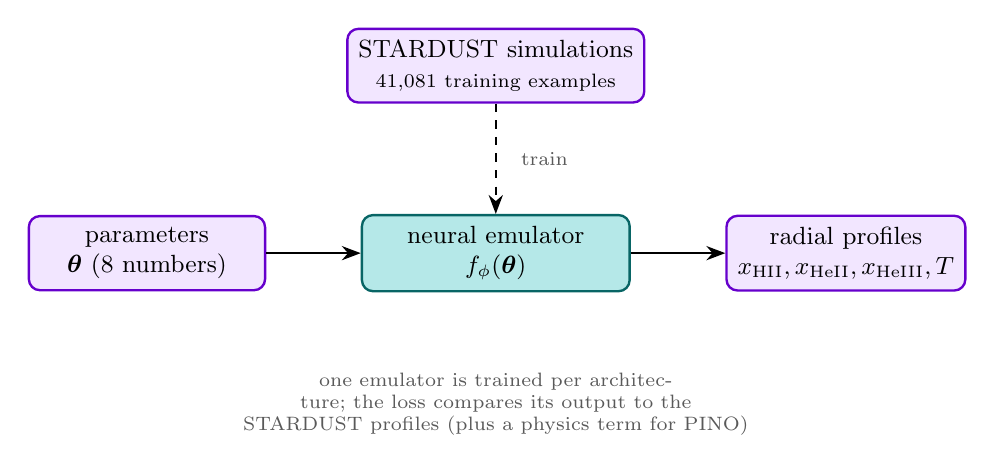
\begin{tikzpicture}[node distance=12mm]
  % main left-to-right flow, boxes given a common width so they align
  \node[data, minimum width=30mm] (in)  {parameters\\$\boldsymbol{\theta}$ (8 numbers)};
  \node[net,  minimum width=34mm, right=of in]  (emu) {neural emulator\\$f_\phi(\boldsymbol{\theta})$};
  \node[data, minimum width=30mm, right=of emu] (out) {radial profiles\\$x_{\rm HII},x_{\rm HeII},x_{\rm HeIII},T$};
  \draw[arr] (in)  -- (emu);
  \draw[arr] (emu) -- (out);

  % training data source, feeding the emulator from above
  \node[data, minimum width=34mm, above=14mm of emu] (sd) {STARDUST simulations\\{\scriptsize 41{,}081 training examples}};
  \draw[darr] (sd) -- node[right, note] {\ \ train} (emu);

  % single clean annotation underneath
  \node[note, below=9mm of emu, text width=72mm]
    {one emulator is trained per architecture; the loss compares its output to the\\
     STARDUST profiles (plus a physics term for PINO)};
\end{tikzpicture}
\end{document}
